
\item In plotting stress versus strain curves for two materials \(P\) and \(Q\), a student by mistake puts strain on the \(y\)-axis and stress on the \(x\)-axis as shown in the figure. Then the correct statement(s) is(are)
        \begin{tasks}(2)
            \task \(P\) has more tensile strength than \(Q\)
            \task \(P\) is more ductile than \(Q\)
            \task \(P\) is more brittle than \(Q\)
            \task The Young's modulus of \(P\) is more than that of \(Q\)
        \end{tasks}
    \begin{center}
        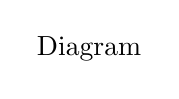
\begin{tikzpicture}
            \node {Diagram};
        \end{tikzpicture}
    \end{center}
